\documentclass[10pt,letterpaper]{article}
\usepackage[top=1in,bottom=1in,left=1in,right=1in]{geometry}
\usepackage{datetime}
\usepackage{natbib}      % http://merkel.zoneo.net/Latex/natbib.php
\usepackage{palatino}
\usepackage{verbatim}
\usepackage[normalem]{ulem}
\bibpunct{(}{)}{;}{a}{,}{,}

\usepackage{enumitem}
\usepackage{array}

\usepackage{chngpage}
\usepackage{stmaryrd}
\usepackage{amssymb}
\usepackage{amsmath}
\usepackage{graphicx}
\usepackage{lscape}
\usepackage{subfigure}
\usepackage[usenames,dvipsnames]{color}
\definecolor{myblue}{rgb}{0,0.1,0.6}
\definecolor{mygreen}{rgb}{0,0.3,0.1}
\usepackage[colorlinks=true,linkcolor=black,citecolor=mygreen,urlcolor=myblue]{hyperref}

\newcommand{\bocomment}[1]{\textcolor{Bittersweet}{BO says: #1}}

\newcommand{\ignore}[1]{}
\newcommand{\transpose}{^\mathsf{T}}
\newcommand{\inner}[1]{\langle #1 \rangle} 
\newcommand{\smallsec}[1]{\noindent \textbf{#1\ }}
\newcommand{\cmd}[1] {{\color{blue}\texttt{#1}}}

\newcommand{\solution}[1]{{\color{myblue} \emph{[Solution:} 

#1 

\emph{End solution]}}}
\newcommand{\solutionnote}[1]{{\color{myblue} \emph{[Note:}

#1 

\emph{End note]}}}
\newcommand{\points}[1]{{\color{mygreen}\emph{[#1]\ \ }}}

\newcommand{\aone}{\diamondsuit}
\newcommand{\atwo}{\heartsuit}
\newcommand{\bone}{\triangle}
\newcommand{\btwo}{\Box}
\newcommand{\myand}{\ \land\ }
\newcommand{\myor}{\ \lor\ }
\newcommand{\mynot}{\lnot}

\title{
  Homework 2 solution template\\
  \Large{CMPSCI 370 Spring 2019, UMass Amherst} \\
  \Large{Name: Subhransu Maji} \\
}


\settimeformat{ampmtime}
\date{}
\begin{document}
\maketitle

\renewcommand\thesubsection{\thesection.\alph{subsection}}

Here is a template that your solutions should roughly follow. Include outputs as figures, and code should be included in the end.

\section{Light}
\begin{enumerate}[label=(\alph*)]
\item Formula for $S_{\text{TOTAL}}$.
\vspace{1in}
\item Tristimulus theory.
	\begin{enumerate}[label=(\arabic*)]
		\item Value of the matrix $R$
		\begin{equation*}
		R=\begin{bmatrix}
			0 & 0 & 0 \\
			0 & 0 & 0 \\
			0 & 0 & 0 
		\end{bmatrix}
		\end{equation*}
		\item Coefficient for the colors
		
		turquoise: $b_1$: \underline{\hspace{3cm}}, $b_2$: \underline{\hspace{3cm}}, $b_3$:\underline{\hspace{3cm}}
		
		goldenrod: $b_1$: \underline{\hspace{3cm}}, $b_2$: \underline{\hspace{3cm}}, $b_3$:\underline{\hspace{3cm}}
	\end{enumerate}
\end{enumerate}


\section{White balance}

\begin{enumerate}
\item Proof for the formula of $L$
\vspace{5in}
\item Value of $L$.

\textbf{Light}~~ $l_r$: \underline{\hspace{2cm}}, $l_g$: \underline{\hspace{3cm}}, $l_b$:\underline{\hspace{3cm}}

\begin{figure}[h]
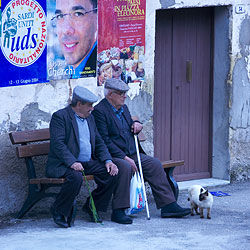
\includegraphics[width=\linewidth]{../data/wb_sardmen-incorrect.jpg}
\caption{Output for the white balance}
\end{figure}

\end{enumerate}

\newpage
\section{Hybrid images} 

$\sigma_1$ = \underline{\hspace{2cm}}, $\sigma_2$ = \underline{\hspace{2cm}}
\begin{figure}[h]
\begin{tabular}{cc}
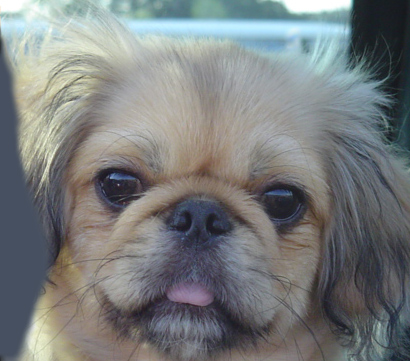
\includegraphics[width=0.48\linewidth]{../output/dog.jpg} &
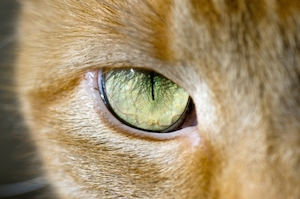
\includegraphics[width=0.48\linewidth]{../output/cat.jpg} \\
dog image & cat image  \\
\end{tabular}
\caption{\label{fig:source} Source images.}
\end{figure}

\begin{figure}[h]
\includegraphics[width=\linewidth]{../output/hybrid-4-10.jpg}
\caption{Output of hybid image of the dog and cat. The image was created with $\sigma_1 = 4$ and $\sigma_2 = 10$.}
\end{figure}


\newpage

\section{Solution code}
Include the source code for your solutions as seen below (only the files you implemented are necessary). 
In latex the command \cmd{verbatiminput\{alignChannels.m\}} allows you to include the code verbatim as seen below. 
Regardless of how you do this the main requirement is that the included code is readable (use proper formatting, variable names, etc.)
A screenshot of your code works too provided you include a link to source files.



\subsubsection{Computing matrix $R$}
\verbatiminput{../initial/computingR}
\subsubsection{Solving $C$}
\verbatiminput{../initial/solving_C}
\subsubsection{grayworld.m}
\verbatiminput{../initial/grayworld}
\subsubsection{hybridImagem}
\verbatiminput{../initial/hybridImage}
\end{document}
